\documentclass[12pt,letterpaper]{article}
\usepackage[utf8]{inputenc}
\usepackage[spanish,es-tabla]{babel}
\decimalpoint
\let\cleardoublepage\clearpage
\usepackage{parskip}
\usepackage{amsmath}
\usepackage{amsfonts}
\usepackage{amssymb}
\usepackage{mathtools}
\usepackage{color}
\usepackage{graphicx}
\usepackage{makeidx}
\usepackage{stanli} % Dibujos SA
% \usepackage{structuralanalysis}
\usepackage{siunitx}
\makeindex
\usepackage{anysize}
\usepackage{anyfontsize}
\usepackage{pdfpages}
\usepackage[x11names,table]{xcolor}
\usepackage{tikz}
\usepackage{tcolorbox}
\tcbuselibrary{skins,breakable,listings,theorems}
\usepackage[hidelinks]{hyperref}
\usepackage[labelfont=bf]{caption}
\usepackage{subcaption}
\usepackage{float}
\captionsetup[table]{labelsep=space}
\captionsetup[figure]{labelsep=space}
\usepackage{setspace} % Para modificar espacios/interlineados
\usepackage{listings}
\usepackage{array,ragged2e}
\usepackage{multirow}
\usepackage[left=1.5cm,top=2cm,right=1.5cm,bottom=2cm]{geometry}
\setlength{\parindent}{0cm}
\usepackage[printwatermark]{xwatermark}
\newwatermark[allpages,color=gray!10,angle=45,scale=3,xpos=0,ypos=0]{Borrador}
\tcbset{colback=green!5!white, colframe=gray!10!black, coltitle=green!20!black, 
fonttitle=\bfseries, colbacktitle=white, coltext=gray!30!black}
\addto\captionsspanish{
  \renewcommand{\figurename}{{\bf Figura}}% 
}
\addto\captionsspanish{
  \renewcommand{\chaptername}{{\bf}}% 
}

\usepackage{epigraph}
\usepackage{fontawesome}
\usepackage[Bjornstrup]{fncychap}

\renewcommand{\baselinestretch}{1.15}

\newcommand{\sifu}[3]{\langle #1 - #2 \rangle^{#3}}

% \renewcommand{\familydefault}{\sfdefault}

% Colores
\definecolor{verdep}{RGB}{166,206,58}
\definecolor{ccap}{RGB}{10,10,50}
\definecolor{csec}{RGB}{50,50,100}
\definecolor{csubsec}{RGB}{80,80,120}
\definecolor{header_table_color}{RGB}{200,255,180}
\definecolor{info_color}{RGB}{100,100,200}
\definecolor{csol}{rgb}{0.2,0.8,0.1}
\definecolor{backcode}{rgb}{0.98,0.98,0.99}
\definecolor{crule}{rgb}{0.9,0.9,0.9}
\definecolor{dkgreen}{rgb}{0,0.6,0}
\definecolor{gray}{rgb}{0.5,0.5,0.5}
\definecolor{mauve}{rgb}{0.58,0,0.82}


\newtcolorbox{ejemplo}[2][]
{
  breakable,
  colframe = gray!100,
  colback  = gray!10,
  coltitle = gray!20!black,
  title    =  \faEdit \hspace{5 mm} #2,
}

\newtcolorbox{informacion}[2][]
{
  breakable,
  colframe = green!5!white,
  colback  = green!5!white,
  coltitle = green!80!black,
  title    = \faInfo \hspace{5 mm} #2,
}

\newtcolorbox{recomendacion}[2][]
{
  breakable,
  colframe = green!25,
  colback  = green!10,
  coltitle = green!20!black,
  title    = #2,
}

\newcolumntype{P}[1]{>{\centering\arraybackslash}m{#1}}
\newcommand{\ccol}{>{\centering\tt\arraybackslash}}

% Nuevos comandos

\usepackage{titlesec}%--
% \newcommand{\hsp}{\hspace{5pt}}
% \titleformat{\chapter}[hang]{\huge\bfseries\color{ccap}}
% {\color{verdep}{\vrule height 2.5cm width 1mm}\hsp{\fontsize{100}{5}\selectfont\thechapter}\hsp%
% {\vrule height 2.5cm width 1mm}\hsp{\fontsize{30}{5}\selectfont}}{5pt}{\huge\bfseries}

\titleformat{\section}[hang]{\normalfont\color{csec}}%
{\filright\large\enspace\thesection\enspace}%
{8pt}{\Large\bfseries\filright}%

\titleformat{\subsection}[hang]{\normalfont\color{csec}}%
{\filright\large\enspace\thesubsection\enspace}%
{8pt}{\large\bfseries\filright}%

% Code
\lstnewenvironment{matlab}{\lstset{frame=single,
  frameround=tttt,
  backgroundcolor=\color{backcode},
  rulecolor=\color{crule},
  language=matlab,
  aboveskip=5mm,
  belowskip=5mm,
  showstringspaces=false,
  columns=flexible,
  basicstyle={\small\ttfamily},
  numbers=none,
  numberstyle=\tiny\color{gray},
  keywordstyle=\color{blue},
  commentstyle=\color{dkgreen},
  stringstyle=\color{mauve},
  breaklines=true,
  breakatwhitespace=true,
  tabsize=4,
  extendedchars=true,
  inputencoding=utf8,
  literate=%
  {°}{{\,\,$^\circ$\,\,}}1
  {á}{{\'a}}1
  {é}{{\'e}}1
  {í}{{\'i}}1
  {ó}{{\'o}}1
  {ú}{{\'u}}1
  {Á}{{\'A}}1
  {É}{{\'E}}1
  {Í}{{\'I}}1
  {Ó}{{\'O}}1
  {Ú}{{\'U}}1
}}{}


\author{
{\small Pedro Jorge De Los Santos}\\[-2mm]
{\small\tt delossantosmfq@gmail.com}
}
\title{
\vspace{-20mm}
{\normalsize Instituto Tecnológico de Celaya} \\[-4mm]
{\normalsize Departamento de Ingeniería Mecánica} \\[-4mm]
{\normalsize Mecánica de Materiales} \\[-4mm]
{\bfseries\normalsize III. Flexión
\footnote{Éstas notas no sustituyen la bibliografía básica, tómelas simplemente como una referencia rápida sobre el contenido 
abordado en la unidad temática correspondiente a Flexión.}
}
}
\date{}

% =================================================================
% =================================================================
%                              CONTENIDO
% =================================================================
% =================================================================

\begin{document}
\maketitle
\tableofcontents


\section{Introducción}

Los elementos estructurales suelen clasificarse de acuerdo con los tipos de
cargas que soportan. Por ejemplo, una barra cargada axialmente soporta
fuerzas con sus vectores dirigidos a lo largo del eje de la barra y una barra
en torsión soporta pares de torsión que tienen sus vectores
momento dirigidos a lo largo del eje. En esta unidad iniciamos nuestro
estudio de las vigas, que son elementos estructurales sometidos
a cargas laterales, es decir, fuerzas o momentos que tienen sus vectores
perpendiculares al eje de la barra.

\section{Tipos de vigas, cargas y apoyos}
  
Las vigas se pueden clasificar de acuerdo con la manera en que se encuentran apoyadas, tal como se muestra 
en la figura \ref{fig:vigas_determinadas}. Note que las reacciones en los soportes de las vigas involucran 
un total de tres incógnitas y pueden determinarse a partir de las ecuaciones de la estática 
($\Sigma F_x =0; \Sigma F_y = 0; \Sigma M =0$).

\begin{figure}[H]
    \centering
    \begin{subfigure}[H]{0.3\textwidth}
        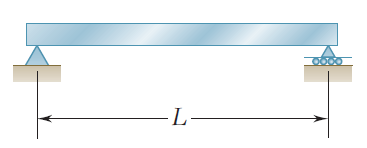
\includegraphics[width=\textwidth]{img/simplemente_apoyada.PNG}
        \caption{Viga simplemente apoyada}
        \label{fig:gull}
    \end{subfigure}
    \begin{subfigure}[H]{0.3\textwidth}
        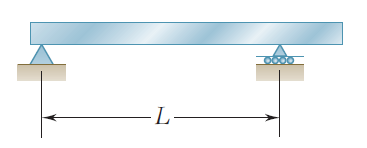
\includegraphics[width=\textwidth]{img/tramo_en_voladizo.PNG}
        \caption{Viga con un tramo en voladizo}
        \label{fig:tiger}
    \end{subfigure}
    \begin{subfigure}[H]{0.3\textwidth}
        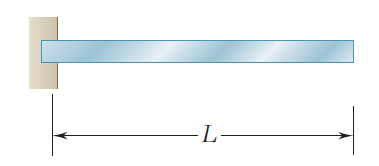
\includegraphics[width=\textwidth]{img/voladizo.PNG}
        \caption{Viga en voladizo}
        \label{fig:mouse}
    \end{subfigure}
    \caption{Vigas estáticamente determinadas}
    \label{fig:vigas_determinadas}
\end{figure}

Existen casos en que las reacciones en las vigas no pueden ser determinadas directamente de las 
ecuaciones de la estática, siendo los más comunes aquellos que se muestran en la figura 
\ref{fig:vigas_indeterminadas}. En estos casos, es necesario conocer adicionalmente el comportamiento 
elástico de la viga cuando se deforma.


\begin{figure}[H]
    \centering
    \begin{subfigure}[H]{0.3\textwidth}
        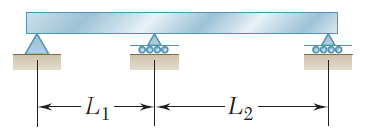
\includegraphics[width=\textwidth]{img/continua.PNG}
        \caption{Viga continua}
        \label{fig:gull}
    \end{subfigure}
    \begin{subfigure}[H]{0.3\textwidth}
        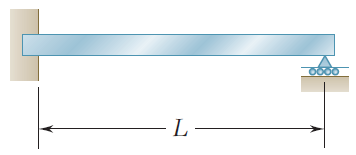
\includegraphics[width=\textwidth]{img/empotrada_apoyada.PNG}
        \caption{Empotrada en un extremo y simplemente apoyada en el otro}
        \label{fig:tiger}
    \end{subfigure}
    \begin{subfigure}[H]{0.3\textwidth}
        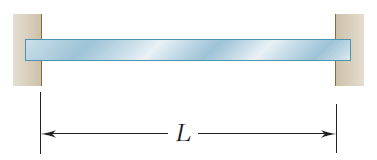
\includegraphics[width=\textwidth]{img/empotrada_doble.PNG}
        \caption{Viga empotrada}
        \label{fig:mouse}
    \end{subfigure}
    \caption{Vigas estáticamente indeterminadas}
    \label{fig:vigas_indeterminadas}
\end{figure}

Existen algunos tipos de cargas comunes en las vigas (ver figura \ref{fig:tipos_cargas}). Las cargas que actúan en una porción 
muy pequeña de una viga son llamadas \textbf{cargas concentradas} o \textbf{cargas puntuales}. 
Las cargas que están \textit{esparcidas} en una porción de la viga se conocen como \textbf{cargas distribuidas}. Las 
cargas distribuidas que son constantes en magnitud son llamadas \textbf{cargas distribuidas uniformes}. En algunos casos 
la carga distribuida puede variar linealmente en la porción que actúa, conociéndose en este caso como \textbf{carga linealmente distribuida}. 
Una viga también puede estar sujeta \textbf{momentos concentrados}, los cuales tienden a flexionar y rotar la viga.

\begin{center}
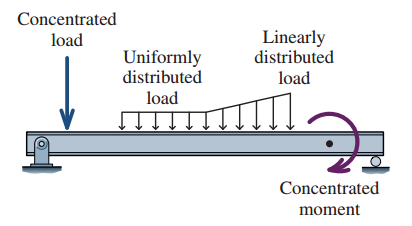
\includegraphics[width=0.5\textwidth]{img/tipos_cargas.PNG}
\captionof{figure}{Tipos de cargas comunes en vigas}
\label{fig:tipos_cargas}
\end{center}



\section{Flexión pura y flexión no uniforme}

Al analizar vigas, con frecuencia es necesario distinguir entre dos casos de flexión:

\begin{itemize}
\item Flexión pura 
\item Flexión no uniforme
\end{itemize}

\textbf{Flexión pura} se refiere a la flexión de una viga ante 
un momento flector constante. Por tanto, la flexión pura ocurre sólo en
regiones de una viga donde la fuerza cortante es cero, una condición derivada 
de las relaciones de cortante y momento que se verán posteriormente. 

Como ejemplo de flexión pura podemos considerar una viga cargada por dos pares $M_1$ que tienen la misma 
magnitud pero que actúan en direcciones opuestas, como se muestra en la figura \ref{fig:flexion_pura}. 
Esa condición de carga produce un momento flexionante constante $M=M_1$ en toda la longitud de la viga.

\begin{center}
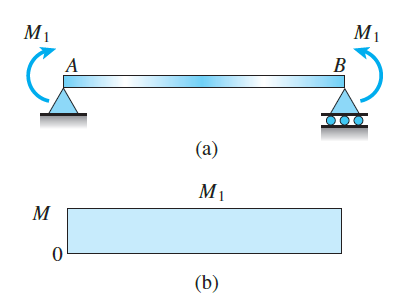
\includegraphics[width=0.5\textwidth]{img/viga_flexion_pura.PNG}
\captionof{figure}{Flexión pura}
\label{fig:flexion_pura}
\end{center}

\textbf{Flexión no uniforme} se refiere a la
flexión en presencia de fuerzas cortantes, lo cual significa que el momento
flexionante cambia conforme nos movemos a lo largo del eje de la viga.

La viga simplemente apoyada de la figura \ref{fig:flexion_no_uniforme} es un ejemplo de una viga que está 
parcialmente en flexión pura y parcialmente en flexión no uniforme, como se observa en los diagramas de 
fuerza cortante y momento flexionante. 

La parte central de la viga está en flexión pura debido a que la fuerza cortante es cero y el momento flector 
constante. Las porciones cercanas a los extremos de la viga están en flexión no uniforme debido a la presencia 
de las fuerzas cortantes y que el momento flexionante es variable.

\begin{center}
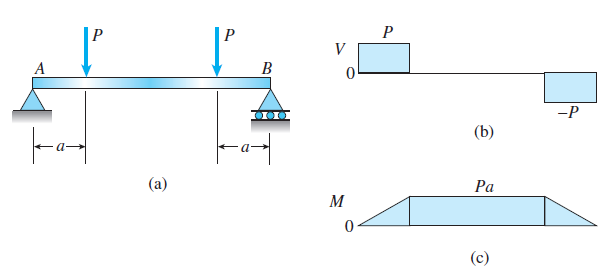
\includegraphics[width=0.75\textwidth]{img/viga_flexion_no_uniforme.PNG}
\captionof{figure}{Flexión no uniforme}
\label{fig:flexion_no_uniforme}
\end{center}


\section{Cortante y momento en vigas: conceptos básicos y diagramas}

Para determinar los esfuerzos desarrollados por la aplicación de cargas, se hace necesario primero determinar 
las fuerzas internas (fuerza cortante $V$ y momento flexionante $M$) que actúan en la viga en cualquier punto de 
interés. El enfoque general para calcular las fuerzas internas se ilustra en la figura \ref{fig:seccionado_viga}, 
una viga simplemente apoyada con un tramo en voladizo está sometida a dos fuerzas puntuales $P_1$ y $P_2$ además de 
una carga distribuida $w$. Un diagrama de cuerpo libre puede obtenerse cortando una sección a una distancia $x$ del 
apoyo en $A$. El plano de corte expone una fuerza cortante interna $V$ y un momento flexionante interno $M$. 
Es importante recordar que si la viga está en equilibrio, entonces cualquier porción de ésta que consideremos cumplirá 
esa condición. Consecuentemente, la porción que se ha cortado deberá estar en equilibrio estático y entonces pueden 
utilizarse esas ecuaciones para determinar los valores para $V$ y $M$ actuando en una coordenada $x$ cualesquiera.

\begin{center}
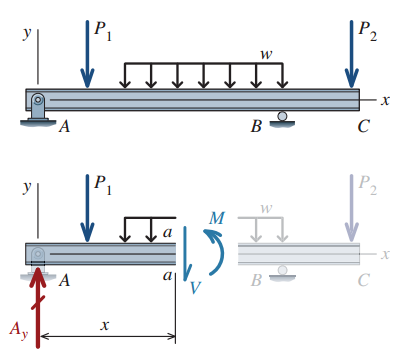
\includegraphics[width=0.45\textwidth]{img/seccionado_viga.PNG}
\captionof{figure}{Seccionado de una viga}
\label{fig:seccionado_viga}
\end{center}

Como se ha mencionado, producto de las fuerzas externas aplicadas las vigas desarrollan fuerzas internas que varían 
a lo largo de la longitud de la viga. Para analizar de manera apropiada los esfuerzos producidos en una viga, es necesario 
determinar el valor de $V$ y $M$ para todos los puntos que definen la longitud de la viga. Lo anterior se gráfica, normalmente, 
en función de la distancia $x$ y suelen llamarse \textbf{diagrama de cortante} y \textbf{diagrama de momento}, estos 
diagramas condensan la información acerca de todas las fuerzas cortantes y momentos flexionantes actuando en la viga, 
haciendo que el trabajo de indentificar los valores máximos para $V$ y $M$ sea más sencillo, luego, esos valores 
extremos son utilizados para calcular los esfuerzos máximos, tanto normales como cortantes.

Dado que habrá diversos tipos de cargas actuando en la viga, las funciones que describen el comportamiento 
del cortante y momento flexionante, $V(x)$ y $M(x)$, pueden no ser continuas en toda la viga. Por ello en muchos 
casos se hace necesario que esas ecuaciones se escriban para los diversos tramos de la viga en forma de 
\textit{funciones a trozos}. Entiéndase por tramos aquellas porciones de la viga que están delimitadas 
por la ubicación de cargas puntuales y reacciones en los apoyos, o bien la porción que ocupa 
una carga distribuida. En la tabla \ref{tab:tramos_vigas} se muestran algunas configuraciones de cargas 
y el número de tramos en cada caso.

% Tabla de propiedades
\begin{table}[H]
\centering
\caption{Vigas y tramos}
\begin{tabular}{P{6cm} P{4cm}} \hline
Disposición de carga & No. de tramos \\
\hline \\
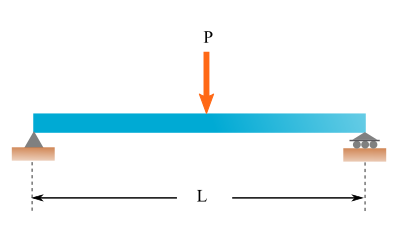
\includegraphics[width=0.3\textwidth]{img/tramo_01.png} & 2 \\
% 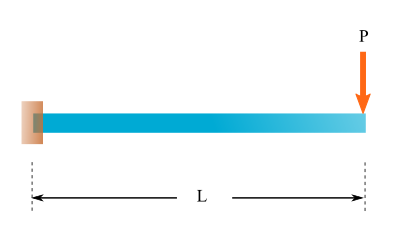
\includegraphics[width=0.3\textwidth]{img/tramo_02.png} & 1 \\
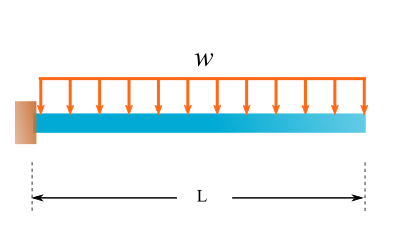
\includegraphics[width=0.3\textwidth]{img/tramo_03.png} & 1 \\
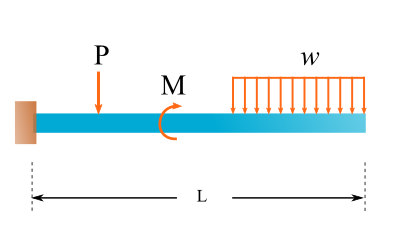
\includegraphics[width=0.3\textwidth]{img/tramo_04.png} & 4 \\
\hline
\end{tabular}
\label{tab:tramos_vigas}
\end{table}

Una consideración importante es la convención de signos a utilizar, ya que permite homogeneizar 
los procedimientos. En general, el cortante $V$ y el momento flector $M$ en un punto dado de 
una viga se consideran positivos cuando las fuerzas internas y los pares que actúan en cada porción 
de la viga se dirigen como se indica en la figura \ref{fig:convencion_signos}a. A modo de 
recordatorio puede advertir lo siguiente:

\begin{itemize}
\item El cortante en cualquier punto de la viga es positivo cuando las fuerzas externas aplicadas 
sobre la viga tienden a cortarla como se muestra en el esquema de la figura \ref{fig:convencion_signos}b.
\item El momento flector en un punto de la viga es positivo cuando las fuerzas externas aplicadas 
sobre la viga tienden a flexionarla como se indica en la figura \ref{fig:seccionado_viga}c.
\end{itemize}

\begin{center}
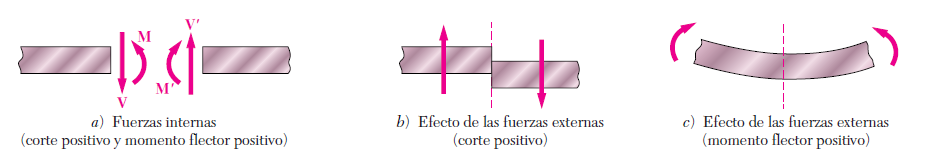
\includegraphics[width=0.95\textwidth]{img/convencion_signos.PNG}
\captionof{figure}{Convención de signos}
\label{fig:convencion_signos}
\end{center}


\subsection{Relaciones entre la carga, el cortante y el momento flector}

Considere una viga simplemente apoyada como la mostrada en la figura \ref{fig:relacion_carga} cargada como se 
indica. Si \textit{cortamos} una sección delimitada por CC' y dibujamos su diagrama de cuerpo libre 
(ver figura \ref{fig:relacion_carga}b), las fuerzas ejercidas sobre el cuerpo libre incluyen una carga de magnitud 
$w \Delta x$ y fuerzas y pares internos en $C$ y en $C'$. Ya que el corte y el momento flector se han supuesto 
positivos, las fuerzas y pares se dirigirán como se indica en la figura \ref{fig:relacion_carga}b.

\begin{center}
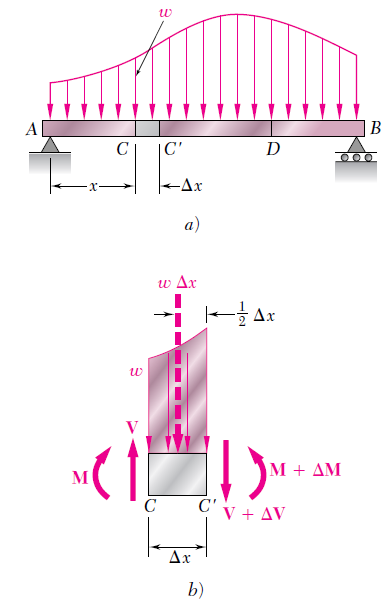
\includegraphics[width=0.45\textwidth]{img/relacion_carga.PNG}
\captionof{figure}{Convención de signos}
\label{fig:relacion_carga}
\end{center}

Indicando que la sumatoria de fuerzas en dirección vertical es cero, se tiene:

$$ V - (V+\Delta V) - w \Delta x = 0 $$
$$ \Delta V = -w \Delta x $$

Dividiendo ambos miembros de la ecuación entre $\Delta x$ y tomando el límite cuando 
$\Delta x \rightarrow 0$, se tiene que:

\begin{equation}\label{eq:rel_cortante}
\frac{dV}{dx} = -w
\end{equation}

La ecuación indica que para una viga cargada como se muestra en la figura \ref{fig:relacion_carga}a, la pendiente 
$dV/dx$ de la curva cortante es negativa; el valor numérico de la pendiente en cualquier punto es igual a la carga 
por unidad de longitud en dicho punto.

Integrando la ecuación anterior entre los puntos C y D se escribe:

\begin{equation}\label{eq:int_cortante}
V_D - V_C = - \int_{x_C}^{x_D} w dx
\end{equation}

$$ V_D - V_C = - (\text{área bajo la cruva de carga entre C y D}) $$

Debe observarse que la ecuacion \ref{eq:rel_cortante} no es válida en un punto donde se aplique 
una carga concentrada, debido a las discontinuidades presentes. Lo mismo aplica para la ecuación 
\ref{eq:int_cortante}, que funcionará sólo para cargas cuya distribución es sucesiva.

Tomando nuevamente como referencia la figura \ref{fig:relacion_carga}, y escribiendo ahora 
que la suma de momentos alrededor de C' es cero, se tiene:

$$ (M+\Delta M) - M - V \Delta x + w \Delta x \frac{\Delta x}{2} = 0 $$
$$ \Delta M = V \Delta x - \frac{1}{2} w (\Delta x)^2 $$

Dividiendo ambos miembros de la ecuación entre $\Delta x$ y tomando el límite cuando 
$\Delta x \rightarrow 0$, se tiene que:

\begin{equation}\label{eq:rel_momento}
\frac{dM}{dx} = V 
\end{equation}

La ecuación \ref{eq:rel_momento} indica que la pendiente $dM/dx$ de la curva de momento flector 
es igual al valor del cortante. Esto es cierto en cualquier punto donde el cortante 
tenga un valor bien definido, esto es, en cualquier punto donde no se encuentre  aplicada una 
carga concentrada. La ecuación \ref{eq:rel_momento} también muestra que $V=0$ en puntos donde 
$M$ es máximo. Esta consideración será muy útil para determinar los posibles puntos críticos 
de la viga.

Integrando la ecuación \ref{eq:rel_momento} entre los puntos C y D se tiene:

\begin{equation}\label{eq:int_momento}
M_D - M_C = \int_{x_C}^{x_D} V \, dx
\end{equation}

$$ M_D - M_C = (\text{área bajo la curva de cortante entre C y D}) $$

Las ecuaciones anteriores todavía son válidas si se aplicada una carga puntual, 
en tanto la curva de momento no tenga discontinuidades. No obstante, si se 
aplica un par dejan de ser válidas, puesto que los pares causan un cambio 
súbito (discontinuidad) en la gráfica del momento flector.


\subsection{Construcción de diagramas de cortante y momento}

Los diagramas de cortante y momento son gráficas en coordenadas rectangulares de las 
funciones cortante $V(x)$ y momento $M(x)$, y como tal se grafica en el eje horizontal 
las coordenada $x$ y en el vertical el valor que toma la función en esa coordenada.

Vamos a tomar un ejemplo básico para mostrar las consideraciones elementales. Suponga 
que tenemos una viga empotrada en un extremo y con un carga concentrada P en el otro, 
como se muestra en la figura.

\begin{center}
\begin{tikzpicture}
    \scaling{4.0}
    \point{a}{0}{0}; 
    \point{b}{1}{0}; 
    \beam{2}{a}{b};
    \load{1}{a}[90];
    \support{3}{b};
    \notation{1}{a}{P}[above=12mm];
    \notation{1}{a}{A}[above left];
    \notation{1}{b}{B};
    \dimensioning{1}{a}{b}{-1.0}[$L$];
\end{tikzpicture}
\end{center}

Si seccionamos podemos obtener que las relaciones para el cortante y momento son:

$$ V = -P $$
$$ M = -Px $$

¿Cómo llevamos estas expresiones a los diagramas de cortante y momento?. Simple, sólo 
considere graficar esas funciones en el intervalo $0 \leq x \leq L$.

Notará que $V$ es una función constante y tendrá por tanto la apariencia de una linea 
recta horizontal ubicada en $V = -P$, considerando que $V$ es la ordenada.

\begin{center}
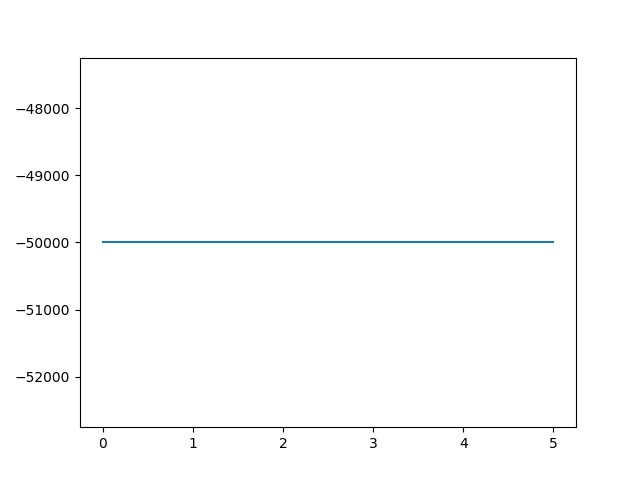
\includegraphics[width=0.45\textwidth]{code/shear.PNG}
\end{center}

En tanto, de $M(x)$ podemos decir que es una función lineal con pendiente negativa (-P) que pasa por 
el origen.

\begin{center}
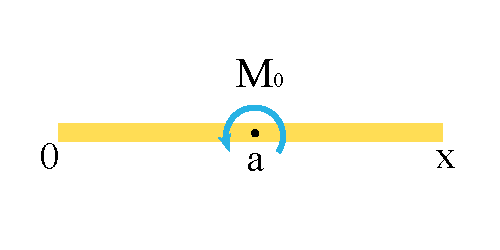
\includegraphics[width=0.45\textwidth]{code/moment.PNG}
\end{center}

Normalmente, se acostumbra a \textit{rellenar} el área entre las curvas y los ejes coordenados, para 
los diagramas de cortante y momento.

\begin{center}
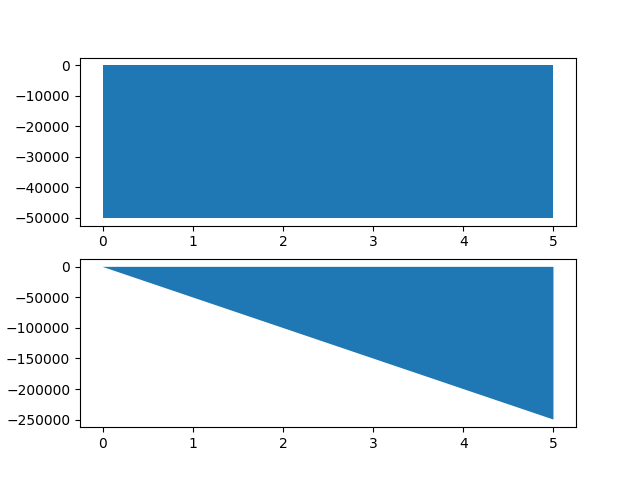
\includegraphics[width=0.45\textwidth]{code/shear_moment.PNG}
\end{center}


\begin{ejemplo}{Ejemplo resuelto}
\textit{Para la viga y carga mostrada en la figura, dibuje los diagramas de cortante y momento}

\begin{center}
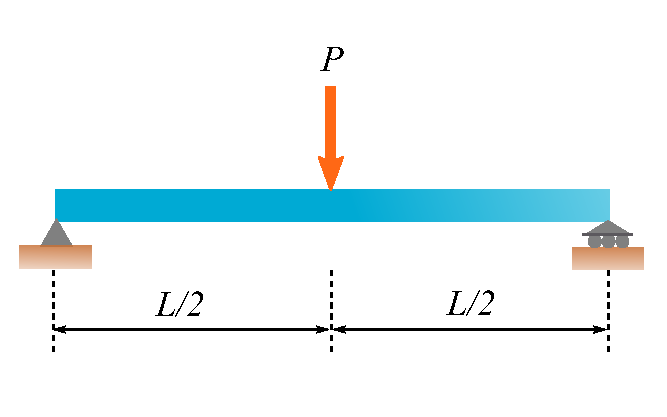
\includegraphics[width=0.5\textwidth]{img/viga_01.pdf}
\end{center}

\textbf{Solución}

Para poder trazar los diagramas de cortante y momento debemos primeramente obtener las expresiones 
correspondientes en cada sección de la viga. Y antes de eso, calcular las reacciones en A y B. Por 
simetría de la carga se tiene que $R_A = R_B$ y están dadas por:

$$ R_A = R_B = P/2 $$

Para la sección A-C ($0 \leq x \leq L/2 $)

\begin{center}
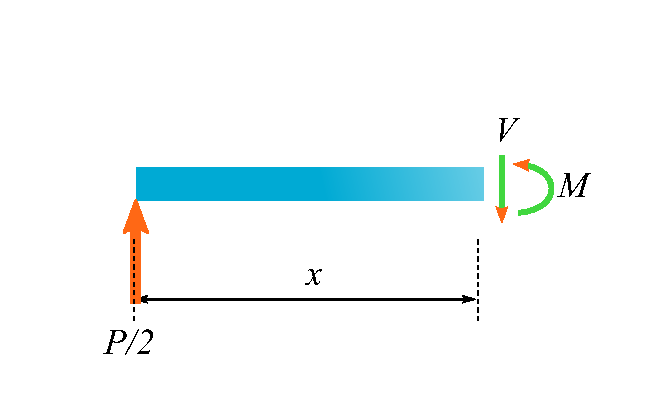
\includegraphics[width=0.45\textwidth]{img/secc_01a.pdf}
\end{center}

$$ +\uparrow \Sigma F_y = 0; \,\,\,\,\, P/2 - V = 0  \,\,\,\, \rightarrow \,\,\,\, V = \frac{P}{2} $$
$$ +\uparrow \Sigma M = 0; \,\,\,\,\,\, -(P/2)(x) + M = 0  \,\,\,\, \rightarrow \,\,\,\, M = \frac{Px}{2} $$


Para la sección C-B ($ L/2 \leq x \leq L $)

\begin{center}
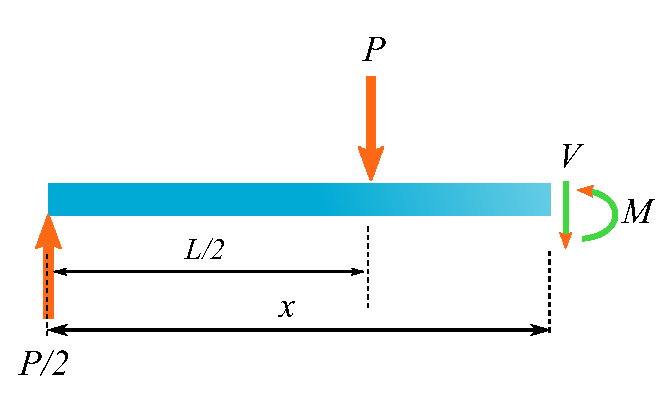
\includegraphics[width=0.45\textwidth]{img/secc_01b.pdf}
\end{center}

$$ +\uparrow \Sigma F_y = 0; \,\,\,\,\, P/2 - P - V = 0  \,\,\,\, \rightarrow \,\,\,\, V = -\frac{P}{2} $$
$$ +\uparrow \Sigma M = 0; \,\,\,\,\,\, -(P/2)(x) + P(x-L/2) + M = 0  \,\,\,\, \rightarrow \,\,\,\, M = -\frac{Px}{2} + \frac{PL}{2} $$

Note que en este caso, al ser una viga compuesta de dos tramos, tanto la función cortante como la de 
momento flector son funciones definidas a trozos, donde:

$$ 
V(x) = \left\{ 
\begin{matrix}
\frac{P}{2} & \text{para  } 0 \leq x \leq L/2 \\
-\frac{P}{2} & \text{para  } L/2 \leq x \leq L \\
\end{matrix}
\right. 
\,\,\,\,\,\,\,\,\,\,\,\,\,\,\,\,
M(x) = \left\{ 
\begin{matrix}
\frac{Px}{2} & \text{para  } 0 \leq x \leq L/2 \\
-\frac{Px}{2} + \frac{PL}{2} & \text{para  } L/2 \leq x \leq L \\ 
\end{matrix}
\right. 
$$


\begin{center}
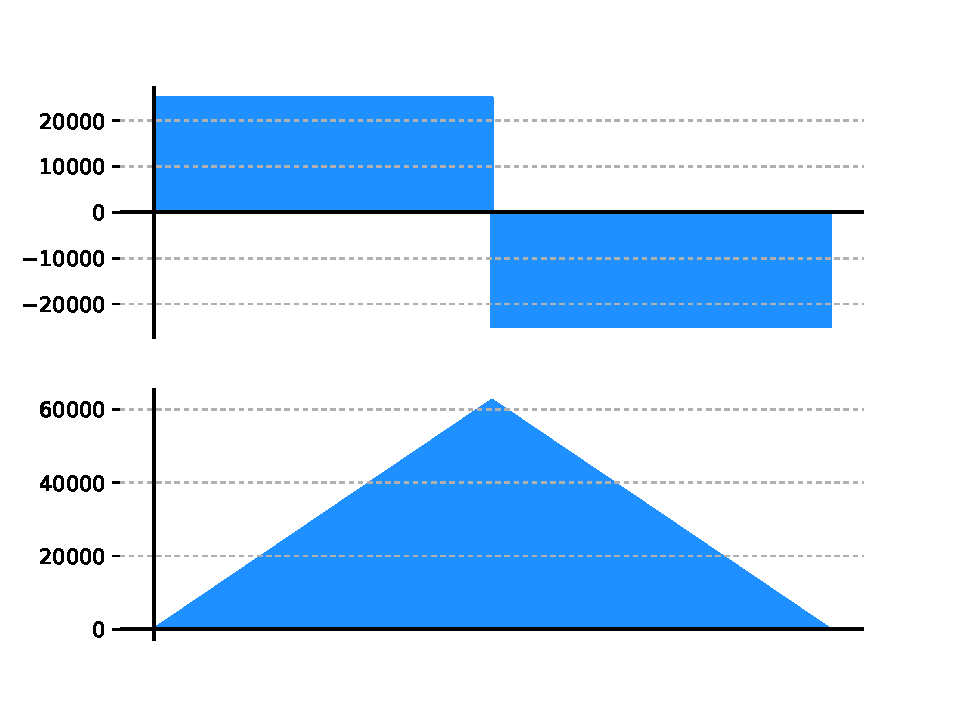
\includegraphics[width=0.6\textwidth]{code/shear_moment_02.pdf}
\end{center}

\end{ejemplo}

\subsubsection{Reglas para trazar diagramas de cortante y momento}

Las que se listan enseguida son recomendaciones que deberá tener en cuenta al 
momento de trazar diagramas de cortante y momento.


\textbf{Reglas para el diagrama de cortante}

\begin{itemize}
\item El diagrama de cortante es discontinuo en los puntos sujetos a fuerzas concentradas $P$. 
Una fuerza $P$ hacia arriba causa que el diagrama de cortante presente un \textit{salto} hacia arriba. 
Una fuerza $P$ hacia abajo causa que el diagrama de cortante presente un \textit{salto} hacia abajo.

\item El cambio en la fuerza de cortante interna entre dos puntos cualesquiera $x_1$ y $x_2$ es 
igual al área bajo la curva de la carga distribuida.

\item En cualquier punto $x$, la pendiente del diagrama de cortante es igual a la intensidad de 
carga distribuida w.
\end{itemize}

\textbf{Reglas para el diagrama de momento}

\begin{itemize}
\item El diagrama de cortante es discontinuo en los puntos sujetos a momentos o pares concentrados $M_O$. 
Un momento $M_O$ en sentido horario causa que el diagrama de momento presente un \textit{salto} hacia arriba. 
Una momento $M_O$ en sentido antihorario causa que el diagrama de cortante presente un \textit{salto} hacia abajo.

\item El cambio en el momento flexionante interno entre dos puntos cualesquiera $x_1$ y $x_2$ es 
igual al área bajo la curva del diagrama de cortante.

\item En cualquier punto $x$, la pendiente del diagrama de momento es igual a la intensidad de 
de la fuerza cortante interna $V$.
\end{itemize}


\textbf{Formas generales de los diagramas}

De manera general, la forma de los diagramas de cortante y momento pueden relacionarse a 
partir de la ecuación:

$$ \frac{dM}{dx} = V $$

$M(x)$ es normalmente una función polinómica de grado $n$, luego, consecuentemente, 
$V(x)$ viene a ser una función polinómica de grado $n-1$. De modo que es relativamente 
sencillo deducir la forma que tendrá una gráfica de momento a partir de la gráfica, 
y viceversa. Si $M(x)$ es un polinomio de grado $n$:

$$ M(x) = a_0 + a_1 x + a_2 x^2 + \cdot + a_n x^n $$

Entonces,

$$ V(x) = a_1 + 2 a_2 x + \cdot + n a_n x^{n-1} $$

\begin{center}
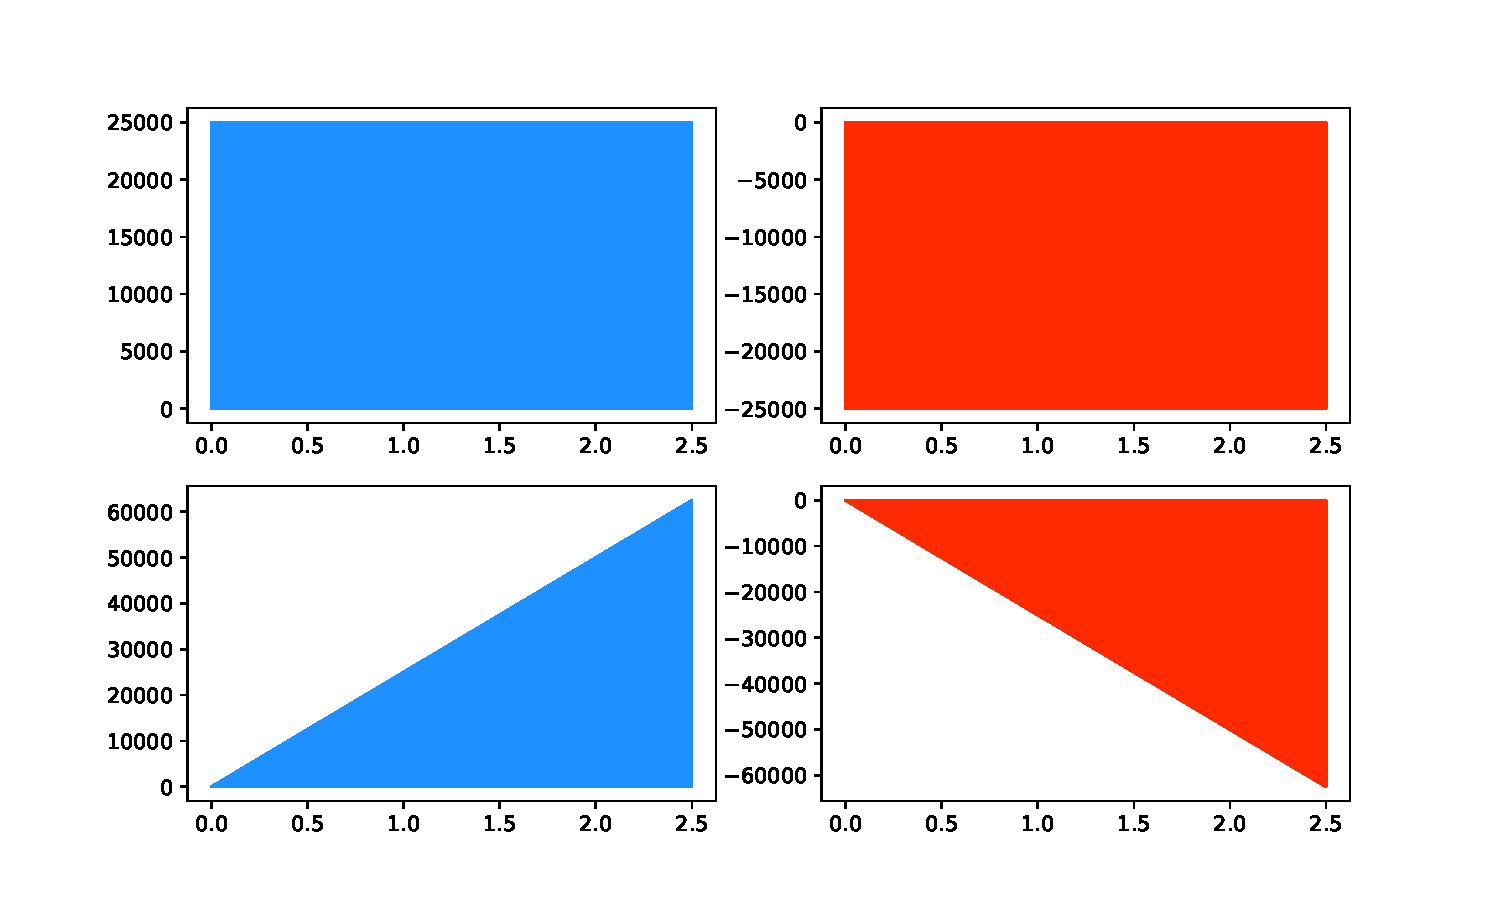
\includegraphics[width=0.75\textwidth]{code/dshape_01.pdf}
\end{center}

\begin{center}
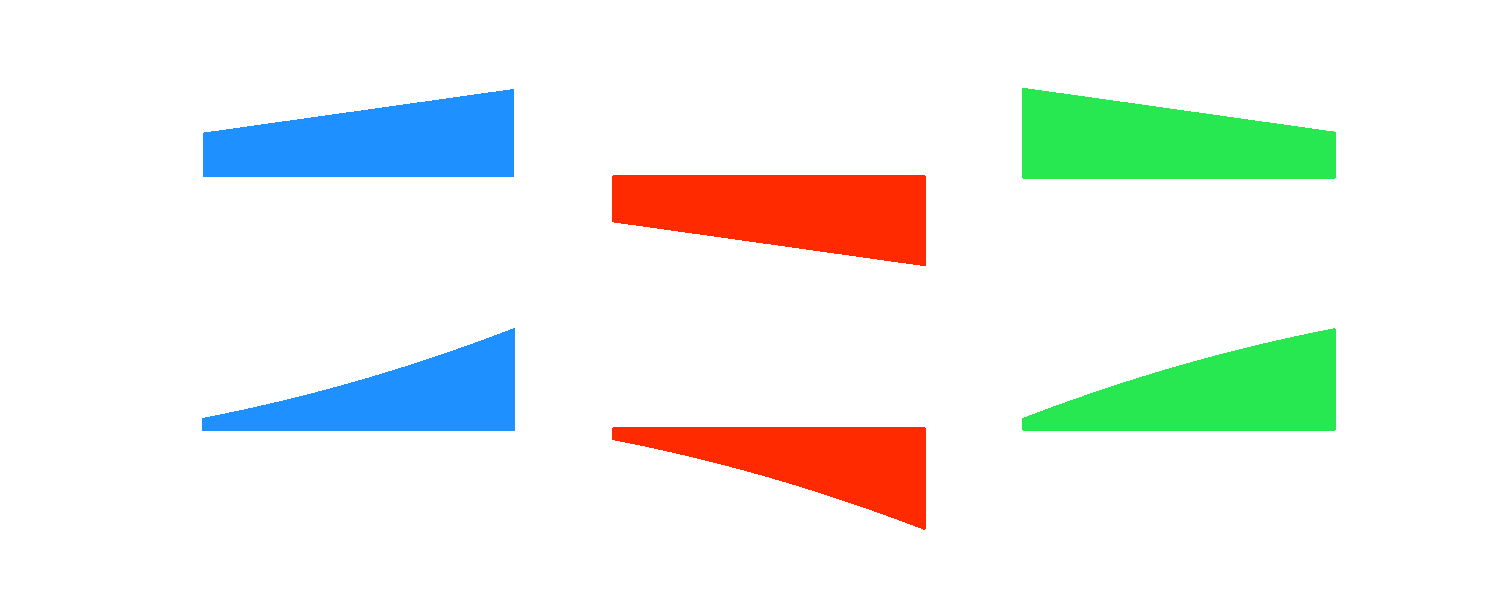
\includegraphics[width=0.75\textwidth]{code/dshape_02.pdf}
\end{center}

De lo anterior, si tenemos una fuerza cortante constante, entonces tendremos una 


\hfill \\[20mm]
\begin{ejemplo}{Ejemplo resuelto}
Una barra de acero de 0.8x2.5 in de sección transversal rectangular está sometida a dos pares iguales y opuestos actuando en el 
plano vertical de simetría de la barra. Calcule el valor del momento flector $M$ que causa la fluencia en la barra. 
Asuma $\sigma_Y = 36 \text{ ksi}$

\begin{center}
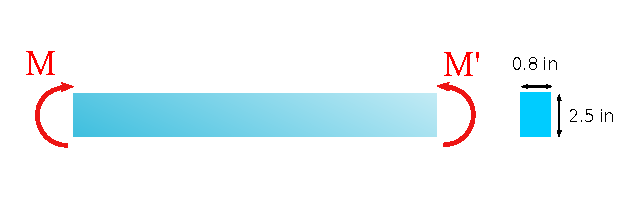
\includegraphics[width=0.75\textwidth]{img/ejemplo_01.pdf}
\end{center}

\textbf{Solución} \\

Dado que el eje neutro pasa a través del centroide de la sección transversal, se tiene que $c=1.25$ in. Además, 
se sabe que el momento de inercia para un área rectangular viene dada por:

$$ I = \frac{1}{12}bh^3 = \frac{1}{12}(0.8)(2.5)^3 = 1.042 \text{ in}^4 $$ 

El esfuerzo máximo para una viga viene dado por:

$$ \sigma_m = \frac{Mc}{I} $$

Luego, el valor de $\sigma_m$ será el valor de la resistencia a la fluencia $\sigma_y$, entonces:

$$ M = \frac{\sigma_m I}{c} = \frac{(1.042)(36x10^3)}{1.25} = 30 \text{ kip*in} $$

\end{ejemplo}



\begin{ejemplo}{Ejemplo resuelto}

Para la viga mostrada en la figura, calcule la deflexión en el punto C. Utilice funciones de singularidad.

\begin{center}
\begin{tikzpicture}
    \scaling{3.0}
    \point{a}{0}{0}; 
    \point{b}{1}{0}; 
    \point{c}{2}{0};
    \beam{2}{a}{b};
    \beam{2}{b}{c};
    \load{1}{b}[90];
    \support{2}{a};
    \support{7}{c};
    \notation{1}{b}{P}[above=12mm];
    \notation{1}{b}{C}[below right];
    \notation{1}{a}{A};
    \notation{1}{c}{B};
    \dimensioning{1}{a}{b}{-1.5}[$L/2$];
    \dimensioning{1}{b}{c}{-1.5}[$L/2$];
\end{tikzpicture}
\end{center}

% \begin{center}
% \begin{tikzpicture}
%     \scaling{3.5}
%     \point{a}{0}{0}; 
%     \point{b}{1}{0}; 
%     \beam{2}{a}{b};
%     \load{1}{a}[270];
%     \load{2}{b};
%     \dimensioning{1}{a}{b}{-1.5}[$x$];
% \end{tikzpicture}
% \end{center}

\textbf{Solución:} \\

Por simetría de la carga, podemos observar que ambas reacciones son iguales y de magnitud equivalente 
a la mitad de la carga puntual aplicada, es decir:

$$ R_A = R_B = \frac{P}{2} $$

Estableciendo la función de carga:

$$ w(x) = - \frac{P}{2} \langle x \rangle^{-1} + P \sifu{x}{\frac{L}{2}}{-1} - \frac{P}{2} \sifu{x}{L}{-1}  $$

Integrando para obtener las expresiones para el cortante y momento:

$$ V(x) = \frac{P}{2} \langle x \rangle^{0} - P \sifu{x}{\frac{L}{2}}{0} $$

$$ M(x) =  \frac{P}{2} \langle x \rangle^{1} - P \sifu{x}{\frac{L}{2}}{1} $$

Podemos escribir la ecuación diferencial para la curva elástica de la viga:

$$ EIy'' = M(x) = \frac{P}{2} \langle x \rangle^{1} - P \sifu{x}{\frac{L}{2}}{1} $$

Integrando e incluyendo las constantes de integración:

$$ EI\theta = \frac{P}{4} \langle x \rangle^{2} - \frac{P}{2} \sifu{x}{\frac{L}{2}}{2} + C_1 $$

$$ EIy = \frac{P}{12} \langle x \rangle^{3} - \frac{P}{6} \sifu{x}{\frac{L}{2}}{3} + C_1 x + C_2 $$

Evaluando la condición de frontera para el apoyo en A, $ [x=0;y=0] $, se tiene que $C_2=0$. \\

Evaluando la condición de frontera para el apoyo en B, $ [x=L;y=0] $, se tiene:

$$ 0 = \frac{P}{12} \langle L \rangle^{3} - \frac{P}{6} \sifu{L}{\frac{L}{2}}{3} + C_1 (L)  $$
$$ 0 = \frac{PL^3}{12} - \frac{PL^3}{48} + C_1 (L)  $$
$$ C_1 = - \frac{PL^2}{16} $$

Entonces, la ecuación de la curva elástica viene dada por:

$$ y = \frac{1}{EI} \left( \frac{P}{12} \langle x \rangle^{3} - \frac{P}{6} \sifu{x}{\frac{L}{2}}{3} - \frac{P L^2 x}{16} \right) $$

Para calcular la deflexión en C basta con hacer $x=L/2$ en la ecuación anterior, tomando en cuenta las 
consideraciones para una función de singularidad:

$$ \Aboxed{ y_C = y(L/2) = - \frac{PL^3}{48} } $$




\end{ejemplo}



\begin{thebibliography}{10}
\bibitem{beer} Beer, F. P. (2013). Mecánica de materiales. México, D.F: McGraw-Hill Interamericana.
\bibitem{gere} Gere, J. M., Goodno, B. J., & León, C. J. (2014). Mecánica de materiales. Australia: Thomson Learning.
\bibitem{gere_timo} Gere, J., & Timoshenko, S. (1998). Mecánica de materiales. México, D.F: Thomson Learning.
\bibitem{hibbeler} Hibbeler, R. C., Murrieta, M. J. E., Molina, S. O., & Saldaña, S. S. (2011). Mecánica de materiales. Naucalpan de Juárez, México: Pearson educación.
\end{thebibliography}


\end{document}